% Beispiel-Filterschaltung:
%
% R2 in Reihe mit R1, R1 parallel zu C
% Eingang u1 über R1 und R2
% Ausgang u2 über R2 bzw. C
% 
% A(omega) = R1 / sqrt( (R1+R2)^2 + (omega C*R1*R2)^2 )
% 
% R1 = 900 Ohm
% R2 = 100 Ohm
% C = 1,25 uF
%
% Amplitudengang linear
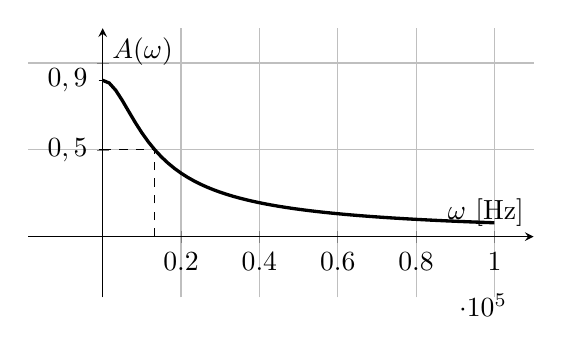
\begin{tikzpicture}
	\begin{axis}[
		xlabel={$\omega\ [\mathrm{Hz}]$},
		ylabel={$A(\omega)$},
		xmin=-19e3, xmax=1.1e5, % xmin < domain_min for yaxis description space
		domain=0:1e5, 
		ymin=-0.35, ymax=1.2,
		samples=61,
		axis x line=center,
		axis y line=center,
		width=8cm,
		height=5cm,
		%ytick={},
		yticklabels={}, % custom as nodes
		ytick distance=0.5,
		grid=major,
	]    
		\addplot[mark=none,very thick,]   {900/(1000^2+(x*100*900*1.25*1e-6)^2)^0.5}; % plot solution from Aufgabe b) A(omega)
			%node[pos=0.4,anchor=south] {$A(\omega)$}; % plotlabel
		\addplot[black,thin] coordinates{(-1e3,0.9)(+1e3,0.9)} node[anchor=east,black] {$0,9\ $}; % yaxis tick
		\addplot[black,thin] coordinates{(-1e3,0.5)(+1e3,0.5)} node[anchor=east,black] {$0,5\ $}; % yaxis tick
		\addplot[dashed,thin] coordinates{(1.3304*1e4,0)(1.3304*1e4,0.5)}; 	% berechnet in aufgabe c)
		\addplot[dashed,thin] coordinates{(0,0.5)(1.3304*1e4,0.5)}; 		% berechnet in aufgabe c)
	\end{axis}
\end{tikzpicture}%
